\chapter{Experimental Boards} \hypertarget{def:eboards}{}

Boards in the experimental phase. Probably with some bugs and missing features. 

\section{Blue Pill}

It is a generic board only with reset, serial and crystal circuits and support to stm32f103c8t6 microcontroller of 
\href{https://beckus.github.io/qemu_stm32/}{qemu-stm32}.

\begin{figure}[H]
\center
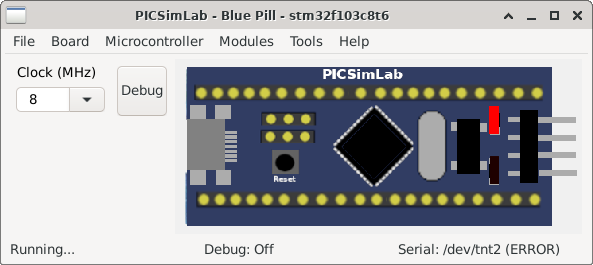
\includegraphics[width=0.7\textwidth]{img/Blue_Pill.png} 
\end{figure} 

\href{https://lcgamboa.github.io/picsimlab_examples/board_Blue_Pill.html}{Examples}


\section{gpboard}

It is a generic board only with reset, serial and crystal circuits and support to multiple microcontrollers 
of \href{http://gpsim.sourceforge.net/}{gpsim}.

\begin{figure}[H]
\center
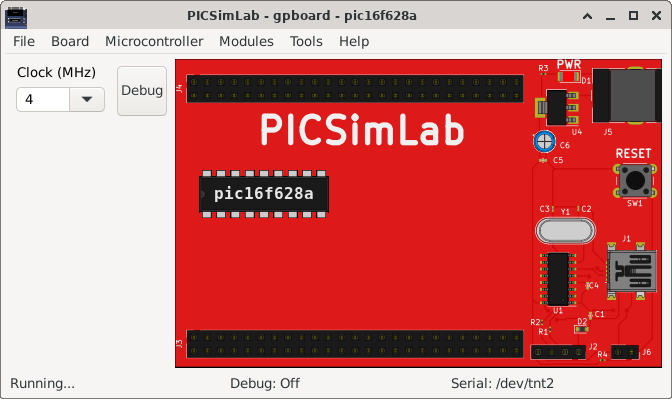
\includegraphics[width=0.7\textwidth]{img/gpboard.png} 
\end{figure} 

\href{https://lcgamboa.github.io/picsimlab_examples/board_gpboard.html}{Examples}


\section{STM32 H103}

It is a generic board only with reset, one push button, serial and crystal circuits and support to stm32f103rbt6 microcontroller of 
\href{https://beckus.github.io/qemu_stm32/}{qemu-stm32}.

\begin{figure}[H]
\center
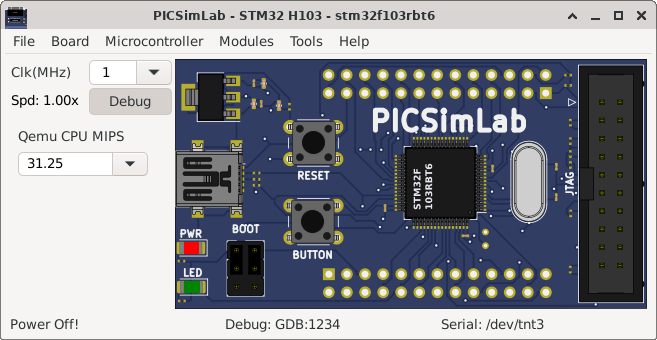
\includegraphics[width=0.7\textwidth]{img/STM32_H103.png} 
\end{figure} 

\href{https://lcgamboa.github.io/picsimlab_examples/board_STM32_H103.html}{Examples}


\section{X}

It is a generic board, used as example in \hrefb{pdf/How to Compile PICsimLab and Create New Boards.pdf}{How to Compile PICsimLab and Create New Boards}.

\begin{figure}[H]
\center
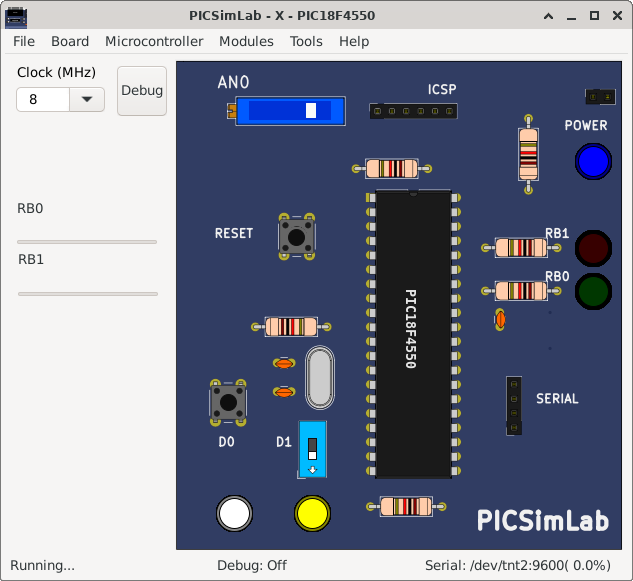
\includegraphics[width=0.7\textwidth]{img/X.png} 
\end{figure} 

\href{https://lcgamboa.github.io/picsimlab_examples/board_X.html}{Examples}

\section{Curiosity }

This is a simple PIC microcontroller development board that uses \href{https://github.com/lcgamboa/picsim}{picsim}.

\begin{figure}[H]
\center
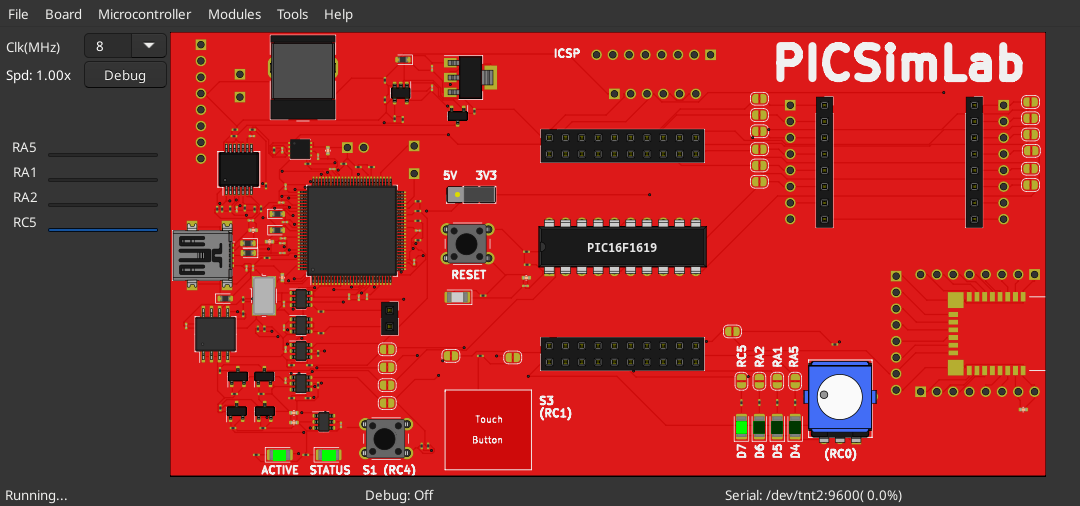
\includegraphics[width=0.7\textwidth]{img/Curiosity.png} 
\end{figure} 

\href{https://lcgamboa.github.io/picsimlab_examples/board_Curiosity.html}{Examples}

\section{Curiosity HPC}

This is a simple PIC microcontroller development board that uses \href{https://github.com/lcgamboa/picsim}{picsim}.

\begin{figure}[H]
\center
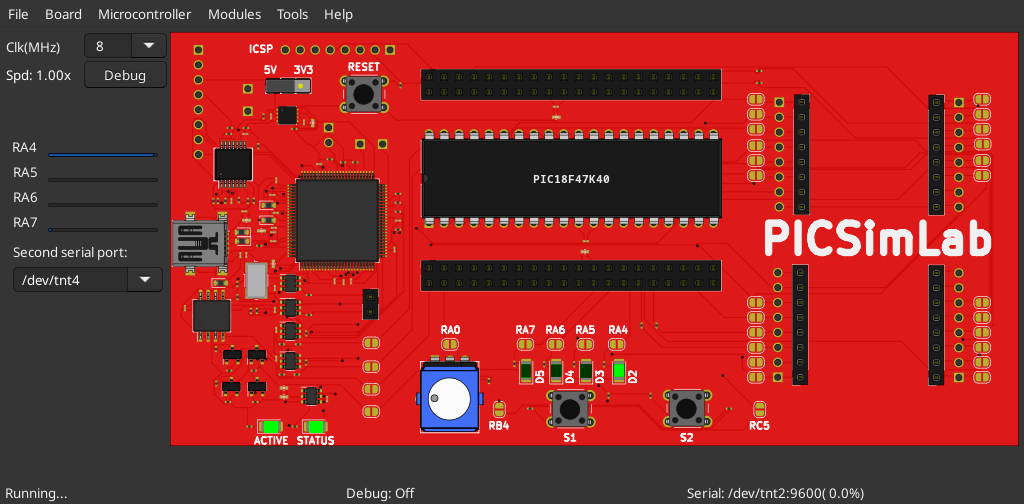
\includegraphics[width=0.7\textwidth]{img/Curiosity_HPC.png} 
\end{figure} 

\href{https://lcgamboa.github.io/picsimlab_examples/board_Curiosity_HPC.html}{Examples}

\section{Xpress}

This is a simple PIC microcontroller development board that uses \href{https://github.com/lcgamboa/picsim}{picsim}.

\begin{figure}[H]
\center
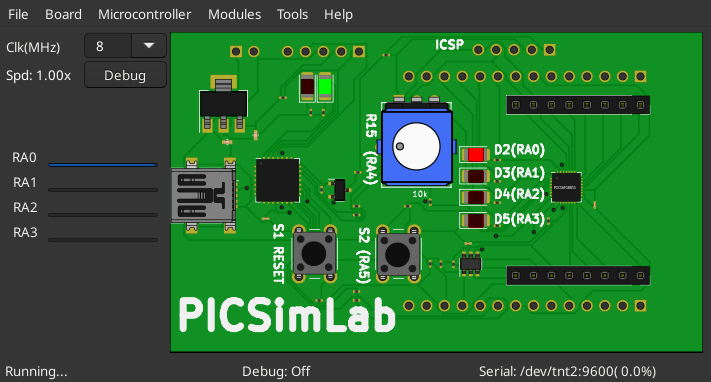
\includegraphics[width=0.7\textwidth]{img/Xpress.png} 
\end{figure} 

\href{https://lcgamboa.github.io/picsimlab_examples/board_Xpress.html}{Examples}


